% Options for packages loaded elsewhere
\PassOptionsToPackage{unicode}{hyperref}
\PassOptionsToPackage{hyphens}{url}
%
\documentclass[
]{article}
\usepackage{amsmath,amssymb}
\usepackage{lmodern}
\usepackage{iftex}
\ifPDFTeX
  \usepackage[T1]{fontenc}
  \usepackage[utf8]{inputenc}
  \usepackage{textcomp} % provide euro and other symbols
\else % if luatex or xetex
  \usepackage{unicode-math}
  \defaultfontfeatures{Scale=MatchLowercase}
  \defaultfontfeatures[\rmfamily]{Ligatures=TeX,Scale=1}
\fi
% Use upquote if available, for straight quotes in verbatim environments
\IfFileExists{upquote.sty}{\usepackage{upquote}}{}
\IfFileExists{microtype.sty}{% use microtype if available
  \usepackage[]{microtype}
  \UseMicrotypeSet[protrusion]{basicmath} % disable protrusion for tt fonts
}{}
\makeatletter
\@ifundefined{KOMAClassName}{% if non-KOMA class
  \IfFileExists{parskip.sty}{%
    \usepackage{parskip}
  }{% else
    \setlength{\parindent}{0pt}
    \setlength{\parskip}{6pt plus 2pt minus 1pt}}
}{% if KOMA class
  \KOMAoptions{parskip=half}}
\makeatother
\usepackage{xcolor}
\usepackage[margin=1in]{geometry}
\usepackage{color}
\usepackage{fancyvrb}
\newcommand{\VerbBar}{|}
\newcommand{\VERB}{\Verb[commandchars=\\\{\}]}
\DefineVerbatimEnvironment{Highlighting}{Verbatim}{commandchars=\\\{\}}
% Add ',fontsize=\small' for more characters per line
\usepackage{framed}
\definecolor{shadecolor}{RGB}{248,248,248}
\newenvironment{Shaded}{\begin{snugshade}}{\end{snugshade}}
\newcommand{\AlertTok}[1]{\textcolor[rgb]{0.94,0.16,0.16}{#1}}
\newcommand{\AnnotationTok}[1]{\textcolor[rgb]{0.56,0.35,0.01}{\textbf{\textit{#1}}}}
\newcommand{\AttributeTok}[1]{\textcolor[rgb]{0.77,0.63,0.00}{#1}}
\newcommand{\BaseNTok}[1]{\textcolor[rgb]{0.00,0.00,0.81}{#1}}
\newcommand{\BuiltInTok}[1]{#1}
\newcommand{\CharTok}[1]{\textcolor[rgb]{0.31,0.60,0.02}{#1}}
\newcommand{\CommentTok}[1]{\textcolor[rgb]{0.56,0.35,0.01}{\textit{#1}}}
\newcommand{\CommentVarTok}[1]{\textcolor[rgb]{0.56,0.35,0.01}{\textbf{\textit{#1}}}}
\newcommand{\ConstantTok}[1]{\textcolor[rgb]{0.00,0.00,0.00}{#1}}
\newcommand{\ControlFlowTok}[1]{\textcolor[rgb]{0.13,0.29,0.53}{\textbf{#1}}}
\newcommand{\DataTypeTok}[1]{\textcolor[rgb]{0.13,0.29,0.53}{#1}}
\newcommand{\DecValTok}[1]{\textcolor[rgb]{0.00,0.00,0.81}{#1}}
\newcommand{\DocumentationTok}[1]{\textcolor[rgb]{0.56,0.35,0.01}{\textbf{\textit{#1}}}}
\newcommand{\ErrorTok}[1]{\textcolor[rgb]{0.64,0.00,0.00}{\textbf{#1}}}
\newcommand{\ExtensionTok}[1]{#1}
\newcommand{\FloatTok}[1]{\textcolor[rgb]{0.00,0.00,0.81}{#1}}
\newcommand{\FunctionTok}[1]{\textcolor[rgb]{0.00,0.00,0.00}{#1}}
\newcommand{\ImportTok}[1]{#1}
\newcommand{\InformationTok}[1]{\textcolor[rgb]{0.56,0.35,0.01}{\textbf{\textit{#1}}}}
\newcommand{\KeywordTok}[1]{\textcolor[rgb]{0.13,0.29,0.53}{\textbf{#1}}}
\newcommand{\NormalTok}[1]{#1}
\newcommand{\OperatorTok}[1]{\textcolor[rgb]{0.81,0.36,0.00}{\textbf{#1}}}
\newcommand{\OtherTok}[1]{\textcolor[rgb]{0.56,0.35,0.01}{#1}}
\newcommand{\PreprocessorTok}[1]{\textcolor[rgb]{0.56,0.35,0.01}{\textit{#1}}}
\newcommand{\RegionMarkerTok}[1]{#1}
\newcommand{\SpecialCharTok}[1]{\textcolor[rgb]{0.00,0.00,0.00}{#1}}
\newcommand{\SpecialStringTok}[1]{\textcolor[rgb]{0.31,0.60,0.02}{#1}}
\newcommand{\StringTok}[1]{\textcolor[rgb]{0.31,0.60,0.02}{#1}}
\newcommand{\VariableTok}[1]{\textcolor[rgb]{0.00,0.00,0.00}{#1}}
\newcommand{\VerbatimStringTok}[1]{\textcolor[rgb]{0.31,0.60,0.02}{#1}}
\newcommand{\WarningTok}[1]{\textcolor[rgb]{0.56,0.35,0.01}{\textbf{\textit{#1}}}}
\usepackage{graphicx}
\makeatletter
\def\maxwidth{\ifdim\Gin@nat@width>\linewidth\linewidth\else\Gin@nat@width\fi}
\def\maxheight{\ifdim\Gin@nat@height>\textheight\textheight\else\Gin@nat@height\fi}
\makeatother
% Scale images if necessary, so that they will not overflow the page
% margins by default, and it is still possible to overwrite the defaults
% using explicit options in \includegraphics[width, height, ...]{}
\setkeys{Gin}{width=\maxwidth,height=\maxheight,keepaspectratio}
% Set default figure placement to htbp
\makeatletter
\def\fps@figure{htbp}
\makeatother
\setlength{\emergencystretch}{3em} % prevent overfull lines
\providecommand{\tightlist}{%
  \setlength{\itemsep}{0pt}\setlength{\parskip}{0pt}}
\setcounter{secnumdepth}{-\maxdimen} % remove section numbering
\ifLuaTeX
  \usepackage{selnolig}  % disable illegal ligatures
\fi
\IfFileExists{bookmark.sty}{\usepackage{bookmark}}{\usepackage{hyperref}}
\IfFileExists{xurl.sty}{\usepackage{xurl}}{} % add URL line breaks if available
\urlstyle{same} % disable monospaced font for URLs
\hypersetup{
  hidelinks,
  pdfcreator={LaTeX via pandoc}}

\author{}
\date{\vspace{-2.5em}}

\begin{document}

\begin{center}\rule{0.5\linewidth}{0.5pt}\end{center}

title: ``Sesión 2. RLM y Supuestos'' subtitle: `Curso: Estadística para
el análisis político 2' date: ``Ciclo 2023-1'' output: pdf\_document:
default html\_document: default latex\_engine: xelatex editor\_options:
markdown: wrap: 72 ---


\includegraphics[width=0.3\linewidth]{logoPUCP}

\hypertarget{regresiuxf3n-lineal}{%
\subsection{Regresión Lineal}\label{regresiuxf3n-lineal}}

LCF: ESTUDIAR LA DATA

\begin{Shaded}
\begin{Highlighting}[]
\FunctionTok{library}\NormalTok{(emo)}
\NormalTok{emo}\SpecialCharTok{::}\FunctionTok{ji}\NormalTok{(}\StringTok{\textquotesingle{}turtle\textquotesingle{}}\NormalTok{)}
\end{Highlighting}
\end{Shaded}

\begin{verbatim}
## 🐢
\end{verbatim}

Consider the emoji: \textbf{lion face, cat, fox face, owl, elephant, sad
face}. I use these symbols in teaching documents to flag a sentence,
paragraph, table or graph as say, something of major importance (lion
face 🦁), question to answer (cat 🐈), suggestion, hint or tip (fox face
🦊), statistical wisdom (owl 🦉), coding conventions \& naming (elephant
🐘) and warning or error (sad face 😟).

emo::ji(``face'')

\hypertarget{ejemplo-1-prediciendo-los-casos-de-covid-19}{%
\subsubsection{Ejemplo 1: Prediciendo los casos de
COVID-19}\label{ejemplo-1-prediciendo-los-casos-de-covid-19}}

Obtenemos nuestra base de datos:

\begin{Shaded}
\begin{Highlighting}[]
\FunctionTok{library}\NormalTok{(rio)}
\NormalTok{competitividad}\OtherTok{=}\FunctionTok{import}\NormalTok{(}\StringTok{"COVID\_COMPETITIVIDAD.sav"}\NormalTok{)}
\FunctionTok{names}\NormalTok{(competitividad)}
\end{Highlighting}
\end{Shaded}

\begin{verbatim}
##  [1] "region"            "casos"             "casos_100k"       
##  [4] "fallecidos"        "poblacion"         "altura"           
##  [7] "pobreza"           "vias_pavimentadas" "var1"             
## [10] "var2"              "var3"              "var4"             
## [13] "var5"              "var6"              "var7"             
## [16] "var8"              "var9"              "var10"            
## [19] "var11"             "var12"             "var13"            
## [22] "var14"             "var15"             "var16"            
## [25] "var17"             "var18"             "var19"            
## [28] "var20"             "var21"             "var22"            
## [31] "var23"             "var24"             "var25"            
## [34] "var26"             "var27"             "var28"            
## [37] "var29"             "var30"             "var31"            
## [40] "var32"             "var33"             "var34"            
## [43] "var35"             "var36"             "var37"            
## [46] "var38"             "var39"             "var40"            
## [49] "var41"             "var42"             "var43"            
## [52] "var44"             "var45"
\end{verbatim}

\hypertarget{recordando-la-regresiuxf3n-lineal}{%
\subsubsection{RECORDANDO LA REGRESIÓN
LINEAL}\label{recordando-la-regresiuxf3n-lineal}}

Calcularemos un modelo para \emph{predecir los casos de COVID-19 a
partir del gasto real por hogar mensual}🥶

Variable dependiente: Casos COVID-19 por cada 100 mil personas
(casos\_100k)

Variable independiente: gasto real por hogar mensual (var5)

\begin{Shaded}
\begin{Highlighting}[]
\NormalTok{modelo }\OtherTok{\textless{}{-}} \FunctionTok{lm}\NormalTok{(competitividad}\SpecialCharTok{$}\NormalTok{casos\_100k }\SpecialCharTok{\textasciitilde{}}\NormalTok{ competitividad}\SpecialCharTok{$}\NormalTok{var5)}
\FunctionTok{summary}\NormalTok{(modelo)}
\end{Highlighting}
\end{Shaded}

\begin{verbatim}
## 
## Call:
## lm(formula = competitividad$casos_100k ~ competitividad$var5)
## 
## Residuals:
##      Min       1Q   Median       3Q      Max 
## -1104.46  -518.17   -93.88   211.99  2263.28 
## 
## Coefficients:
##                      Estimate Std. Error t value Pr(>|t|)    
## (Intercept)         -994.9169   695.3350  -1.431 0.167188    
## competitividad$var5    2.1284     0.5086   4.185 0.000418 ***
## ---
## Signif. codes:  0 '***' 0.001 '**' 0.01 '*' 0.05 '.' 0.1 ' ' 1
## 
## Residual standard error: 743.8 on 21 degrees of freedom
## Multiple R-squared:  0.4547, Adjusted R-squared:  0.4287 
## F-statistic: 17.51 on 1 and 21 DF,  p-value: 0.0004178
\end{verbatim}

Seguimos nuestro flujograma para evaluar el modelo:

\begin{enumerate}
\def\labelenumi{\arabic{enumi}.}
\tightlist
\item
  Nos preguntamos si el modelo es válido
\item
  Qué tanto explica el modelo:
\item
  Si la variable independiente aporta al modelo
\item
  Identificamos los coeficientes
\end{enumerate}

¿Qué sucede si ahora agregamos más variables?

\#insertamos meme

Calculamos nuestro modelo, en este caso usaremos lo siguiente:

Variable dependiente: Casos COVID-19 por cada 100 mil personas Variables
independientes: Stock de capital por trabajador (var3) + gasto real por
hogar mensual (var5) + morbilidad (var20).

\begin{Shaded}
\begin{Highlighting}[]
\NormalTok{modelo1 }\OtherTok{\textless{}{-}} \FunctionTok{lm}\NormalTok{(competitividad}\SpecialCharTok{$}\NormalTok{casos\_100k}\SpecialCharTok{\textasciitilde{}}\NormalTok{ competitividad}\SpecialCharTok{$}\NormalTok{var3}\SpecialCharTok{+}\NormalTok{competitividad}\SpecialCharTok{$}\NormalTok{var5}\SpecialCharTok{+}
\NormalTok{               competitividad}\SpecialCharTok{$}\NormalTok{var20)}
\CommentTok{\#otra forma de usar la función lm (usando menos símbolos de $), sería la siguiente:}
\CommentTok{\#modelo1 \textless{}{-} lm(casos\_100k\textasciitilde{} var3+var5+var20, competitividad)}
\FunctionTok{summary}\NormalTok{(modelo1)}
\end{Highlighting}
\end{Shaded}

\begin{verbatim}
## 
## Call:
## lm(formula = competitividad$casos_100k ~ competitividad$var3 + 
##     competitividad$var5 + competitividad$var20)
## 
## Residuals:
##     Min      1Q  Median      3Q     Max 
## -800.31 -360.70    8.18  340.91 1331.92 
## 
## Coefficients:
##                        Estimate Std. Error t value Pr(>|t|)   
## (Intercept)           1.811e+03  1.206e+03   1.501  0.14986   
## competitividad$var3   2.382e-02  8.178e-03   2.913  0.00892 **
## competitividad$var5   1.484e+00  4.165e-01   3.563  0.00207 **
## competitividad$var20 -3.678e+01  1.550e+01  -2.373  0.02833 * 
## ---
## Signif. codes:  0 '***' 0.001 '**' 0.01 '*' 0.05 '.' 0.1 ' ' 1
## 
## Residual standard error: 548.8 on 19 degrees of freedom
## Multiple R-squared:  0.7314, Adjusted R-squared:  0.689 
## F-statistic: 17.25 on 3 and 19 DF,  p-value: 1.185e-05
\end{verbatim}

Seguimos nuestro flujograma para evaluar el modelo:

\begin{enumerate}
\def\labelenumi{\arabic{enumi}.}
\tightlist
\item
  Nos preguntamos si el modelo es válido:
\end{enumerate}

\begin{itemize}
\tightlist
\item
  Si el p-value es menor a 0.05 significa que rechazamos la hipótesis
  nula, lo cual probaría que nuestro modelo sí funciona.
\end{itemize}

-Al tener un p-value de 1.185e-05 nuestro modelo sí funciona.

\begin{enumerate}
\def\labelenumi{\arabic{enumi}.}
\setcounter{enumi}{1}
\tightlist
\item
  ¿Qué tanto explica el modelo? -Revisamos el R cuadrado ajustado que va
  de 0 a 1 (0\% a 100\%)
\end{enumerate}

-En este caso mis variables (en conjunto) explican el 68.9\% de la
variabilidad de mi dependiente, esto es bueno, pero quizá podría ser
mejor.

\begin{enumerate}
\def\labelenumi{\arabic{enumi}.}
\setcounter{enumi}{2}
\tightlist
\item
  ¿Las variables independientes aportan al modelo? -Nos enfocamos en el
  p-value de cada independiente
\end{enumerate}

-corroboramos que estas rechazen la hipótesis nula, es decir que sean
menores que 0.05.

\begin{enumerate}
\def\labelenumi{\arabic{enumi}.}
\setcounter{enumi}{3}
\tightlist
\item
  Identificamos los coeficientes -En este caso hacemos uso del código
  modelo1\$coefficients.
\end{enumerate}

-Armamos nuestra ecuación: y=1810.55+ var3*(0.02382484)+
var5(1.48405800) + var20(-36.78156990)

\#install.packages(``lm.beta'')

\begin{Shaded}
\begin{Highlighting}[]
\FunctionTok{library}\NormalTok{(lm.beta)}
\NormalTok{modelo1}\SpecialCharTok{$}\NormalTok{coefficients}
\end{Highlighting}
\end{Shaded}

\begin{verbatim}
##          (Intercept)  competitividad$var3  competitividad$var5 
##        1810.55164809           0.02382484           1.48405800 
## competitividad$var20 
##         -36.78156990
\end{verbatim}

\hypertarget{supuestos}{%
\subsubsection{SUPUESTOS}\label{supuestos}}

\hypertarget{linealidad-el-problema-es-la-no-linealidad}{%
\subsubsection{1- Linealidad (el problema es la no
linealidad)}\label{linealidad-el-problema-es-la-no-linealidad}}

\textbf{Descrición} Como su nombre lo dice, debe de existir una
linealidad entre la variable independiente y dependiente, en otras
palabras,la linealidad indica que el valor esperado de la variable
dependiente es una función lineal de cada variable independiente,
manteniendo las demás fijas. La pendiente de esa línea no depende de los
valores de las otras variables, por ello también nos fijamos variable
por variable. Los efectos de diferentes variables independientes sobre
el valor esperado de la variable dependiente son aditivos. Si este
supuesto no se cumple significaría que posiblemente existan variables
que no aporten al modelo o que se trate de una relación no lineal.

\textbf{Cómo detectarlo}

OPCIÓN 1: Exploración gráfica: Plot de valores residuales frente a
valores predichos.

OPCIÓN 2: Calculando la correlación bivariada de cada independiente con
la dependiente.

\textbf{Código e interpretación}

\begin{Shaded}
\begin{Highlighting}[]
\FunctionTok{library}\NormalTok{(ggfortify)}
\end{Highlighting}
\end{Shaded}

\begin{verbatim}
## Loading required package: ggplot2
\end{verbatim}

\begin{Shaded}
\begin{Highlighting}[]
\CommentTok{\#Exploración gráfica}
\FunctionTok{plot}\NormalTok{(modelo1,}\DecValTok{1}\NormalTok{)}
\end{Highlighting}
\end{Shaded}

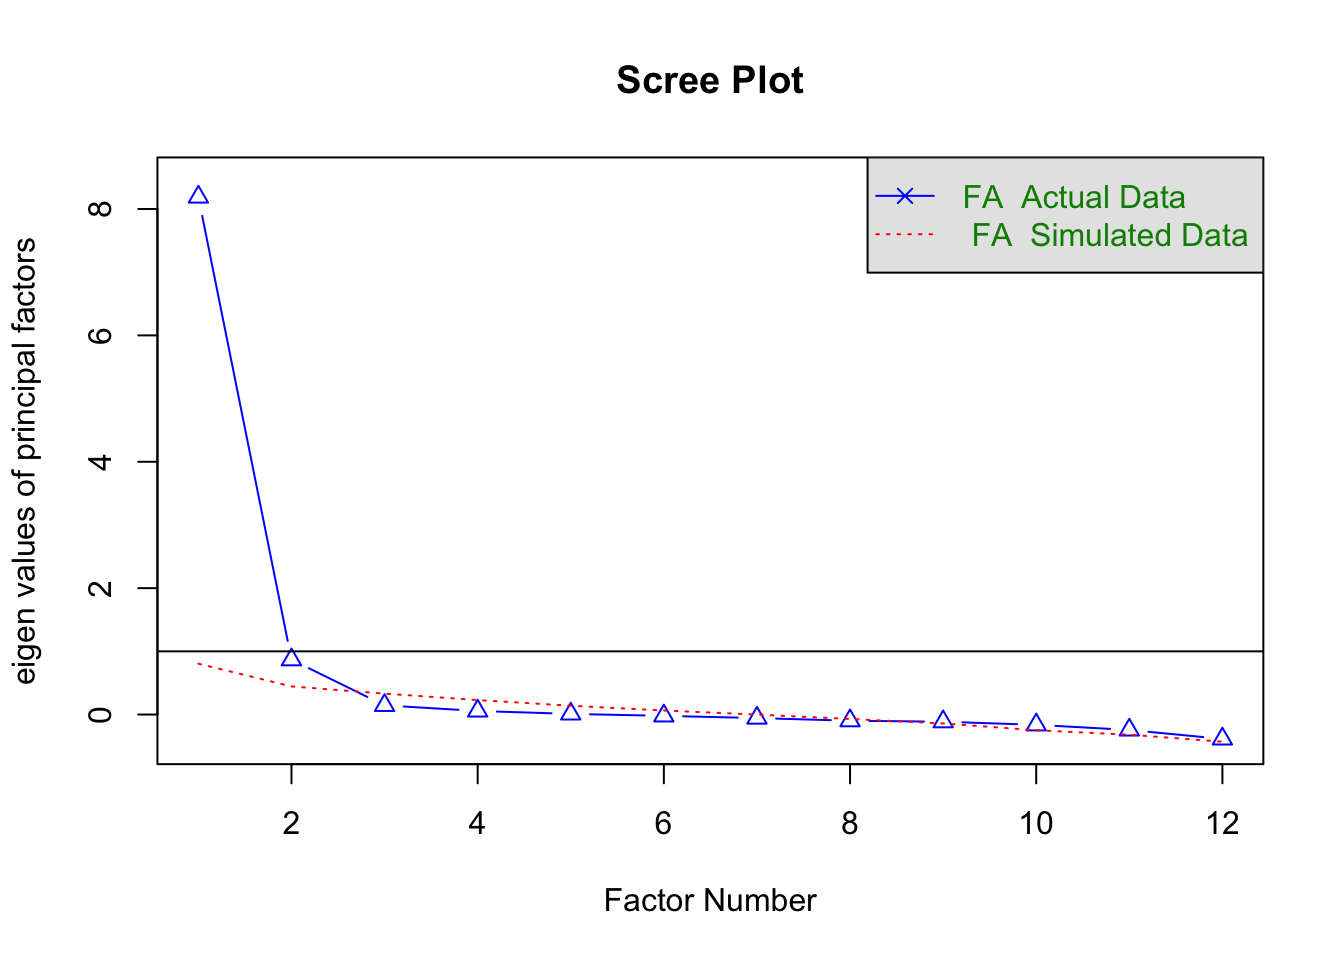
\includegraphics{Sesión2-_RLMySupuestos_files/figure-latex/unnamed-chunk-7-1.pdf}

\begin{Shaded}
\begin{Highlighting}[]
\FunctionTok{autoplot}\NormalTok{(modelo1,}\DecValTok{1}\NormalTok{)}
\end{Highlighting}
\end{Shaded}

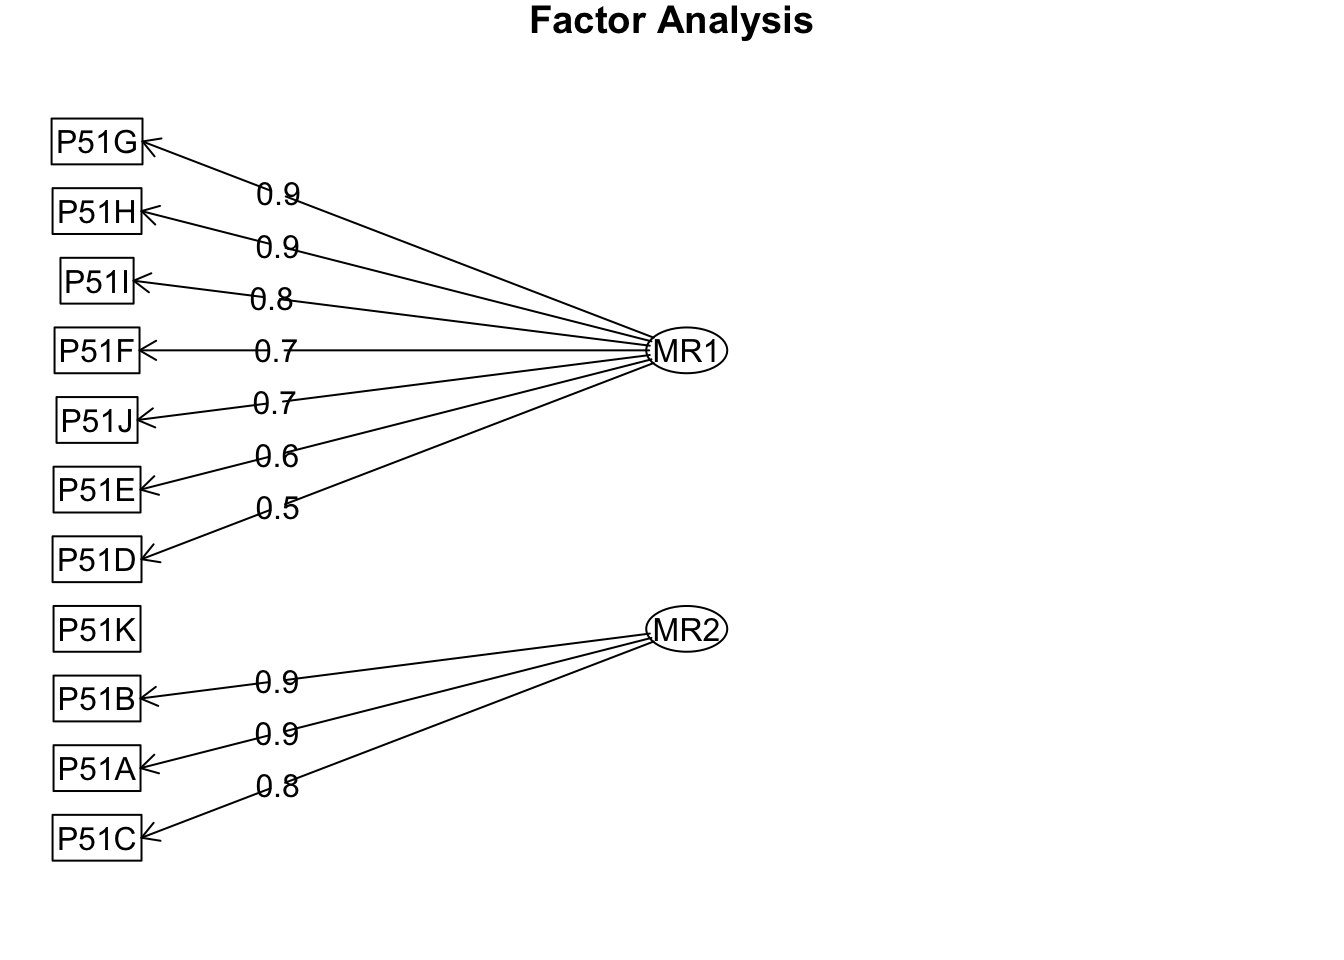
\includegraphics{Sesión2-_RLMySupuestos_files/figure-latex/unnamed-chunk-7-2.pdf}

Usando el código plot, la línea roja debería de estar lo más cercana a
la línea punteada. De acuerdo al resultado, el gráfico aún nos generaría
suspicacias. En tanto, dado que la línea roja obedece a los puntos,
éstos deberían distribuirse alrededor de una línea horizontal, con una
varianza aproximadamente constante.

Si usamos la correlación, entonces revisamos cada una de las variables:
-Nos fijamos en el p-value -Nos fijamos en el cor

\begin{Shaded}
\begin{Highlighting}[]
\CommentTok{\#Usando el test}
\FunctionTok{cor.test}\NormalTok{(competitividad}\SpecialCharTok{$}\NormalTok{casos\_100k, competitividad}\SpecialCharTok{$}\NormalTok{var3)}
\end{Highlighting}
\end{Shaded}

\begin{verbatim}
## 
##  Pearson's product-moment correlation
## 
## data:  competitividad$casos_100k and competitividad$var3
## t = 4.3943, df = 21, p-value = 0.0002531
## alternative hypothesis: true correlation is not equal to 0
## 95 percent confidence interval:
##  0.3916650 0.8592019
## sample estimates:
##       cor 
## 0.6921267
\end{verbatim}

\begin{Shaded}
\begin{Highlighting}[]
\FunctionTok{cor.test}\NormalTok{(competitividad}\SpecialCharTok{$}\NormalTok{casos\_100k, competitividad}\SpecialCharTok{$}\NormalTok{var5)}
\end{Highlighting}
\end{Shaded}

\begin{verbatim}
## 
##  Pearson's product-moment correlation
## 
## data:  competitividad$casos_100k and competitividad$var5
## t = 4.1847, df = 21, p-value = 0.0004178
## alternative hypothesis: true correlation is not equal to 0
## 95 percent confidence interval:
##  0.3630301 0.8502056
## sample estimates:
##      cor 
## 0.674325
\end{verbatim}

\begin{Shaded}
\begin{Highlighting}[]
\FunctionTok{cor.test}\NormalTok{(competitividad}\SpecialCharTok{$}\NormalTok{casos\_100k, competitividad}\SpecialCharTok{$}\NormalTok{var20)}
\end{Highlighting}
\end{Shaded}

\begin{verbatim}
## 
##  Pearson's product-moment correlation
## 
## data:  competitividad$casos_100k and competitividad$var20
## t = -2.3995, df = 21, p-value = 0.02578
## alternative hypothesis: true correlation is not equal to 0
## 95 percent confidence interval:
##  -0.7354473 -0.0638803
## sample estimates:
##        cor 
## -0.4638681
\end{verbatim}

Al revisar todas las variables nos damos cuenta que todas tienen un
p-value menor a 0.05, lo cual nos da a conocer que sí existe relación
lineal.Sin embargo, si tuviese que sacar una variable, podría ser la
var20, que a pesar de que sí cumple con un p-value menor que 0.05 (se
rechaza la hipótesis nula), de todas las variables es la más cercana a
``no cumplir''.

También lo puedes graficar para que te de una idea de forma más rápida:

\#install.packages(``corrplot'')

\begin{Shaded}
\begin{Highlighting}[]
\FunctionTok{library}\NormalTok{(corrplot)}
\end{Highlighting}
\end{Shaded}

\begin{verbatim}
## corrplot 0.92 loaded
\end{verbatim}

\begin{Shaded}
\begin{Highlighting}[]
\CommentTok{\#La funci?n cor calcula la matriz de correlaciones}
\NormalTok{M}\OtherTok{\textless{}{-}}\FunctionTok{cor}\NormalTok{(competitividad[,}\FunctionTok{c}\NormalTok{(}\DecValTok{3}\NormalTok{,}\DecValTok{11}\NormalTok{,}\DecValTok{13}\NormalTok{,}\DecValTok{28}\NormalTok{)],}\AttributeTok{method=}\StringTok{"pearson"}\NormalTok{)}
\FunctionTok{corrplot}\NormalTok{(M, }\AttributeTok{method=}\StringTok{"circle"}\NormalTok{,}\AttributeTok{type=}\StringTok{"upper"}\NormalTok{)}
\end{Highlighting}
\end{Shaded}

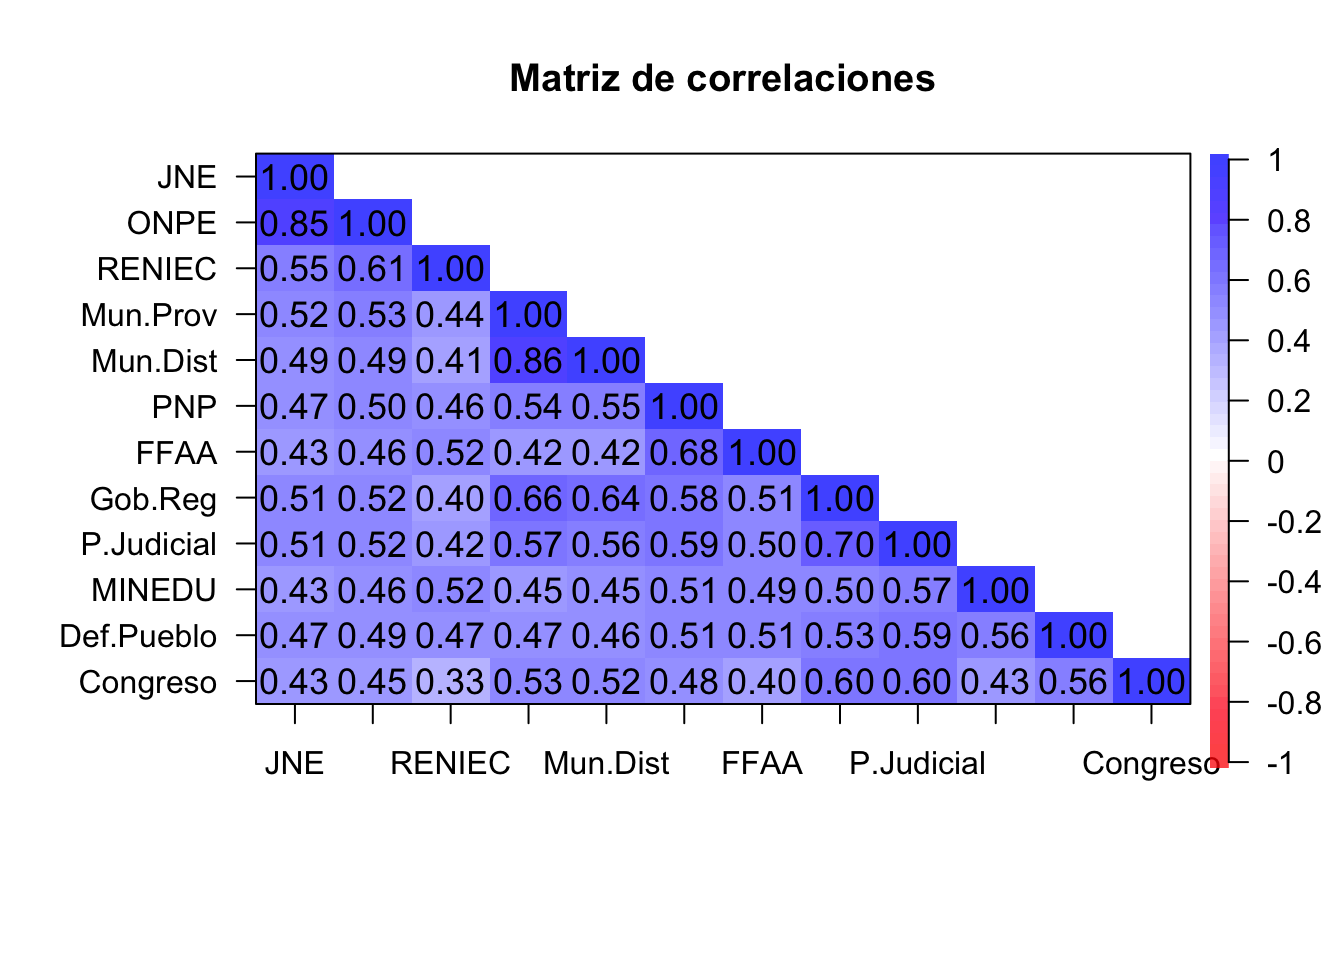
\includegraphics{Sesión2-_RLMySupuestos_files/figure-latex/unnamed-chunk-9-1.pdf}

\begin{Shaded}
\begin{Highlighting}[]
\FunctionTok{corrplot}\NormalTok{(M, }\AttributeTok{method=}\StringTok{"number"}\NormalTok{)}
\end{Highlighting}
\end{Shaded}

\includegraphics{Sesión2-_RLMySupuestos_files/figure-latex/unnamed-chunk-9-2.pdf}

\begin{Shaded}
\begin{Highlighting}[]
\FunctionTok{corrplot.mixed}\NormalTok{(M)}
\end{Highlighting}
\end{Shaded}

\includegraphics{Sesión2-_RLMySupuestos_files/figure-latex/unnamed-chunk-9-3.pdf}

\hypertarget{normalidad-de-residuos-el-problema-es-la-no-normalidad}{%
\subsubsection{2. Normalidad de residuos (el problema es la NO
normalidad)}\label{normalidad-de-residuos-el-problema-es-la-no-normalidad}}

\textbf{Descrición}

Identificar si los errores siguen una distribución normal. La resta del
valor observado menos el valor pronosticado (residuos) siguen una
distribución normal, esto es importante porque si es que no se cumple no
se podrían aplicar las pruebas globales del modelo.

\textbf{Cómo detectarlo}

Exploración gráfica: QQ plot de residuos Pruebas de normalidad a los
residuos. Normalmente bastaría con la prueba de Shapiro Wilk, pero
también se pueden probar otros como Lillieford, Kolmogorov (no es muy
exigente), entre otros.

\textbf{Código e interpretación}

Si usamos sólo gráfico

\begin{Shaded}
\begin{Highlighting}[]
\FunctionTok{plot}\NormalTok{(modelo1, }\DecValTok{2}\NormalTok{) }\CommentTok{\#o también se puede usar el código autoplot(modelo1,2), las dos indicarían lo mismo.}
\end{Highlighting}
\end{Shaded}

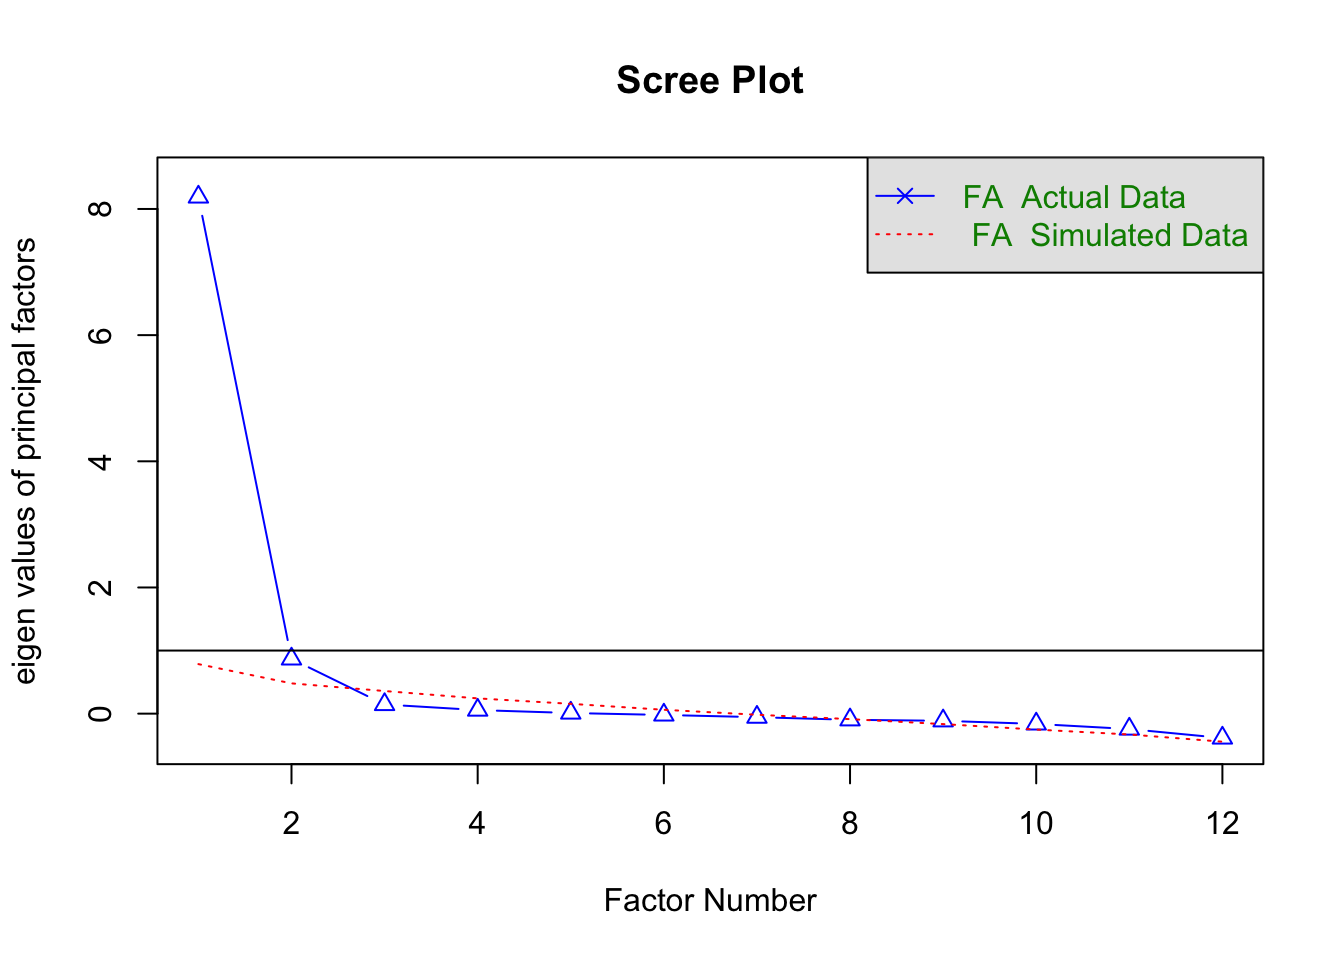
\includegraphics{Sesión2-_RLMySupuestos_files/figure-latex/unnamed-chunk-10-1.pdf}

\begin{Shaded}
\begin{Highlighting}[]
\FunctionTok{library}\NormalTok{(ggfortify)}
\FunctionTok{autoplot}\NormalTok{(modelo1,}\DecValTok{2}\NormalTok{)}
\end{Highlighting}
\end{Shaded}

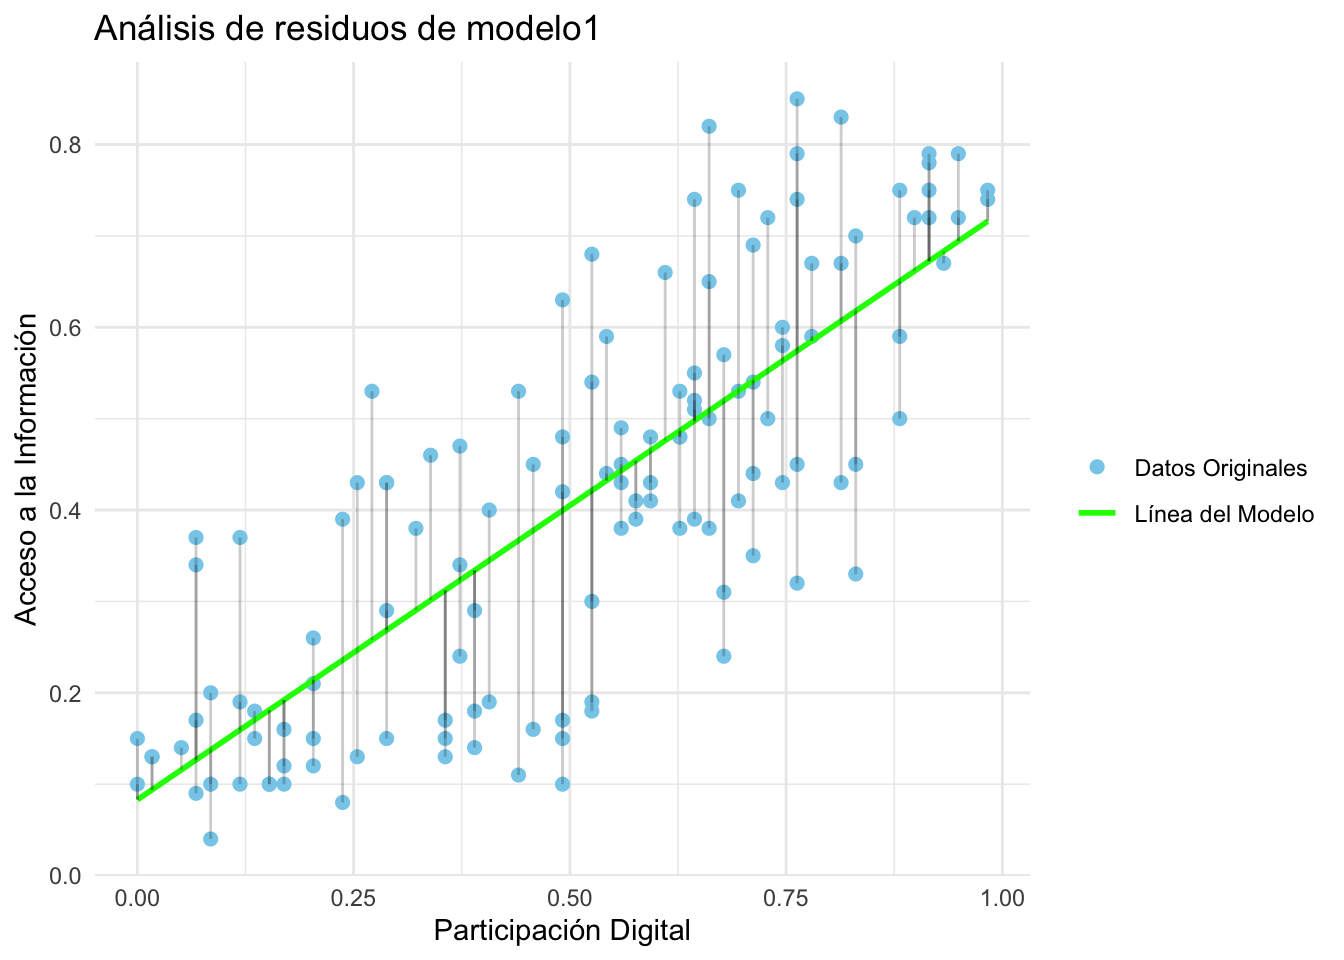
\includegraphics{Sesión2-_RLMySupuestos_files/figure-latex/unnamed-chunk-11-1.pdf}

Todos los puntos deben estar sobre la diagonal. Los dos gráficos no son
concluyentes, entonces procedo a realizar el test.

Si usamos prueba de normalidad:aplicamos la prueba de Shapiro a los
residuos del modelo

\begin{Shaded}
\begin{Highlighting}[]
\FunctionTok{shapiro.test}\NormalTok{(modelo1}\SpecialCharTok{$}\NormalTok{resid)}
\end{Highlighting}
\end{Shaded}

\begin{verbatim}
## 
##  Shapiro-Wilk normality test
## 
## data:  modelo1$resid
## W = 0.96627, p-value = 0.6006
\end{verbatim}

Ojo con la hipótesis nula. H0: Es normal (distribución normal)
\textbar{} Ha: No es normal (no hay distribución normal)

Si el pvalor es menor a 0.05 entonces NO existe normalidad de residuos
(problemas!), se rechazaría la distribución normal. Dado que nuestro
p-value es 0.6006, mayor que 0.05, entonces sí estamos frente a un caso
de distribució normal de los residuos.

\hypertarget{homocedasticidad-el-problema-es-la-heterocedasticidad}{%
\subsubsection{3- Homocedasticidad (el problema es la
heterocedasticidad)}\label{homocedasticidad-el-problema-es-la-heterocedasticidad}}

\textbf{Descrición}

La homocedasticidad (también conocido como homogeneidad en la varianza
de los residuos) indica que las variancias de los errores son
constantes. Cuando no se cumple es un problema porque los estimadores no
son consistentes ni eficientes y se presenta el caso de la
heterocedasticidad.

\textbf{Cómo detectarlo}

OPCIÓN 1: Exploración gráfica: diagrama de residuos standarizados y
valores predichos.

OPCIÓN 2: Con el Score Test for Non-Constant Error Variance, también
llamado Test Breusch Pagan. Evalúa si la varianza del error cambia con
el nivel de la variable respuesta (valores ajustados) o con una
combinación lineal de predictores.

\textbf{Código e interpretación}

Si usamos el gráfico

\begin{Shaded}
\begin{Highlighting}[]
\FunctionTok{plot}\NormalTok{(modelo1, }\DecValTok{3}\NormalTok{)}
\end{Highlighting}
\end{Shaded}

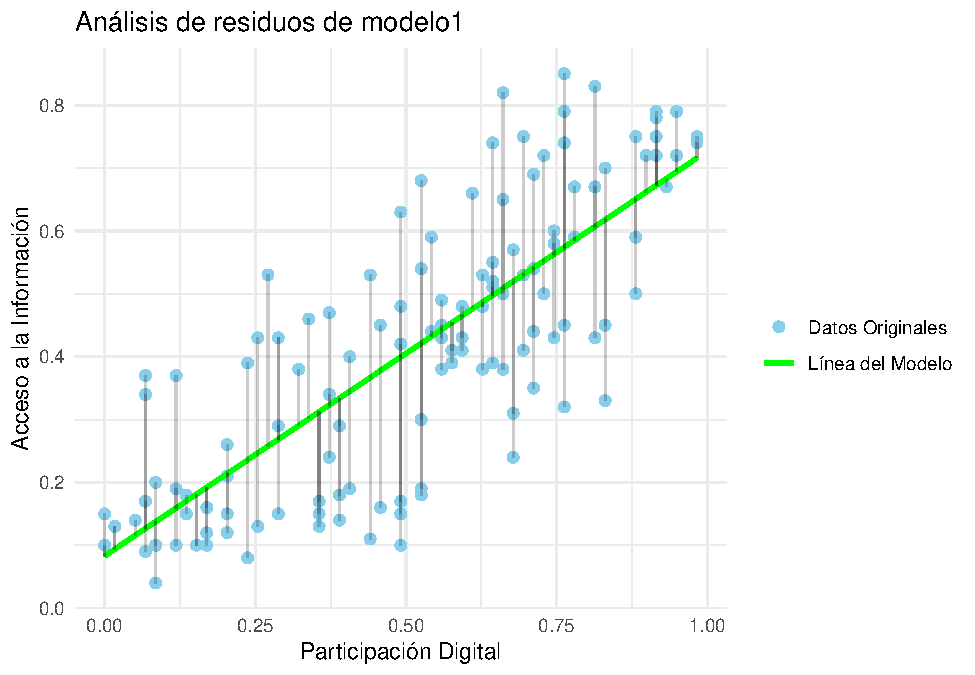
\includegraphics{Sesión2-_RLMySupuestos_files/figure-latex/unnamed-chunk-13-1.pdf}

En el Gráfico la línea roja debe seguir una tendencia horizontal, esto
representaría que la distribución de los puntos son uniformes. Al ver
nuestro gráfico nos damos cuenta que la línea roja va hacia arriba, lo
cual nos dice que el gráfico no es concluyente aún. Vamos al test.

Si usamos el test de BP:

\begin{Shaded}
\begin{Highlighting}[]
\FunctionTok{library}\NormalTok{(lmtest)}
\FunctionTok{bptest}\NormalTok{(modelo1)}
\end{Highlighting}
\end{Shaded}

\begin{verbatim}
## 
##  studentized Breusch-Pagan test
## 
## data:  modelo1
## BP = 1.6987, df = 3, p-value = 0.6372
\end{verbatim}

H0: El modelo es homocedástico Ha: El modelo es heterocedástico

Si el pvalor es menor a 0.05 entonces el modelo es heterocedástico
(problema!). Esta vez estamos frente a un modelo homocedástico

\hypertarget{ausencia-de-multicolinealidad-el-problema-es-la-presencia-de-multicolinealidad}{%
\subsubsection{4. Ausencia de multicolinealidad (el problema es la
presencia de
multicolinealidad)}\label{ausencia-de-multicolinealidad-el-problema-es-la-presencia-de-multicolinealidad}}

\textbf{Descripción}

Se aplica en la regresión lineal MÚLTIPLE. Significa que las variables
explicativas están relacionadas linealmente entre sí. La
multicolinealidad hace que los coeficientes del modelo se vuelvan
inestables, es decir, oscilarán violentamente ante cambios mínimos en
las variables de insumo. Esto entendería que existe una relación fuerte
entre variables independientes, por lo tanto podría darnos un modelo
inestable.

\textbf{Cómo detectarlo}

Con el Factor de Inflación de Varianza (VIF). los factores de inflación
de varianza deben de ser menores de 5. De acuerdo a nuestros resultados
no encontramos multicolinealidad.

\textbf{Código e interpretación}

\begin{Shaded}
\begin{Highlighting}[]
\FunctionTok{library}\NormalTok{(DescTools)}
\FunctionTok{VIF}\NormalTok{(modelo1)}
\end{Highlighting}
\end{Shaded}

\begin{verbatim}
##  competitividad$var3  competitividad$var5 competitividad$var20 
##             1.337011             1.231735             1.098254
\end{verbatim}

Valores \textgreater{} 5 indican presencia de multicolinealidad.

\hypertarget{independencia-de-residuos-el-problema-es-que-existe-autocorrelaciuxf3n-en-los-residuos}{%
\subsubsection{5.- Independencia de residuos (el problema es que existe
autocorrelación en los
residuos)}\label{independencia-de-residuos-el-problema-es-que-existe-autocorrelaciuxf3n-en-los-residuos}}

\textbf{Descripción}

Si los errores residuales \textbf{no son independientes}, es probable
que demuestren algún tipo de patrón (que no siempre es obvio a simple
vista).

\textbf{Cómo detectarlo}

Se puede realizar el Test de Durbin Watson (que mide el la presencia de
correlación de cada error residual con el error residual ``anterior'')

\textbf{Código e interpretación}

\begin{Shaded}
\begin{Highlighting}[]
\CommentTok{\#Default}
\FunctionTok{library}\NormalTok{(car)}
\FunctionTok{durbinWatsonTest}\NormalTok{(modelo1)}
\end{Highlighting}
\end{Shaded}

\begin{verbatim}
##  lag Autocorrelation D-W Statistic p-value
##    1     -0.04132242      1.743747   0.482
##  Alternative hypothesis: rho != 0
\end{verbatim}

Durbin Watson: Las hipótesis son: H0: Los residuos son independientes
Ha: Los residuos no son independientes Si el pvalor es menor a 0.05
entonces los residuos no son independientes o también se podría decir
que están \textbf{autocorrelacionados} (problema!). En este caso tenemos
un p value de 0.518, mayor a 0.05, el cual nos indica que no nos
encontramos frente a un caso de autocorrelación.

\textbf{Modelo 2} ¿Es posible mejorar mi modelo1? Esta vez, realizamos
una regresión sin nuestra var20.

\begin{Shaded}
\begin{Highlighting}[]
\NormalTok{modelo2 }\OtherTok{\textless{}{-}} \FunctionTok{lm}\NormalTok{(casos\_100k}\SpecialCharTok{\textasciitilde{}}\NormalTok{ var3}\SpecialCharTok{+}\NormalTok{var5, competitividad)}
\FunctionTok{summary}\NormalTok{(modelo2)}
\end{Highlighting}
\end{Shaded}

\begin{verbatim}
## 
## Call:
## lm(formula = casos_100k ~ var3 + var5, data = competitividad)
## 
## Residuals:
##    Min     1Q Median     3Q    Max 
## -885.0 -351.2 -192.7  419.9 1446.0 
## 
## Coefficients:
##               Estimate Std. Error t value Pr(>|t|)   
## (Intercept) -7.773e+02  5.730e+02  -1.357  0.19004   
## var3         2.930e-02  8.708e-03   3.365  0.00308 **
## var5         1.455e+00  4.620e-01   3.150  0.00504 **
## ---
## Signif. codes:  0 '***' 0.001 '**' 0.01 '*' 0.05 '.' 0.1 ' ' 1
## 
## Residual standard error: 609 on 20 degrees of freedom
## Multiple R-squared:  0.6518, Adjusted R-squared:  0.617 
## F-statistic: 18.72 on 2 and 20 DF,  p-value: 2.62e-05
\end{verbatim}

Seguimos nuestro flujograma para evaluar el modelo:

\begin{enumerate}
\def\labelenumi{\arabic{enumi}.}
\tightlist
\item
  Nos preguntamos si el modelo es válido:
\end{enumerate}

\begin{itemize}
\tightlist
\item
  Si el p-value es menor a 0.05 significa que rechazamos la hipótesis
  nula, lo cual probaría que nuestro modelo sí funciona. -Al tener un
  p-value de 2.62e-05 nuestro modelo sí funciona.
\end{itemize}

\begin{enumerate}
\def\labelenumi{\arabic{enumi}.}
\setcounter{enumi}{1}
\tightlist
\item
  ¿Qué tanto explica el modelo? -Revisamos el R cuadrado ajustado que va
  de 0 a 1 (0\% a 100\%) -En este caso mis variables (en conjunto)
  explican el 61.7\% de la variabilidad de mi dependiente, esto es
  bueno, pero quizá podría ser mejor.
\item
  ¿Las variables independientes aportan al modelo? -Nos enfocamos en el
  p-value de cada independiente -corroboramos que estas rechazen la
  hipótesis nula, es decir que sean menores que 0.05.
\end{enumerate}

Conclusiones preliminares: el modelo sí pasa la evaluación; mis
variables siguen aportando al modelo, mi modelo es válido al tener un p
value de 2.62e-05; sin embargo, al sacar la variable var20 nos damos
cuenta que mi modelo2 explica menos que mi modelo1. Por lo tanto, solo
al evaluar mi modelo2, a pesar de que es un modelo válido, optaría por
mantener mi modelo1. Ojo, solo basándome en esta primera evaluación del
modelo. Una decisión más fina sería al realizar mis pruebas de supuestos
completa.

\end{document}
